\chapter{Background and Related Works}\label{background}

    This chapter aims to introduce background knowledge that relates to this project including deep neural network, android development, and distance calculation.
    Then, this chapter gives examples of related works.

    \section{Deep Neural Network}
        A Deep Neural Network (DNNs) is a deep learning's architecture,
        which is a part of machine learning, and it is based on artificial intelligence.
        DNN is stimulated from the human nervous system, which contains cells.
        These cells are called neurons, and they are fully linked \cite{deep-learing-2}.
        Likewise, DNNs are composed of multiple layers between input and output,
        and each layer has neurons, which are entirely connected \cite{deep-learing-3}.
        These layers turn input to output by passing data through each layer and doing some computation,
        and this is called forward propagation \cite{deep-learing-2}, \cite{deep-learing-1}.
        DNN can be applied in many fields such as computer vision (CV), speech recognition, or object detection \cite{deep-learing-1}.


    \section{Threading in Android}
        Threads in Android development are split into two main categories: the main thread and a worker thread.
        A main thread or UI thread is a thread that dispatch events of user interface widgets.
        The events are dispatched regarding Android's activity lifecycle,
        and all events are managed by only one thread.
        In other words, threads will not be spawned for handling a single event or component.
        Thus, if there is a long-running task, which is run by UI thread, events cannot be delivered
        because long-running task block UI thread.
        If UI thread is blocked more than 5 seconds,
        an application will show "Application not Responding"  \cite{ANDROID-01}.

        \begin{figure}[!ht]
            \centering
            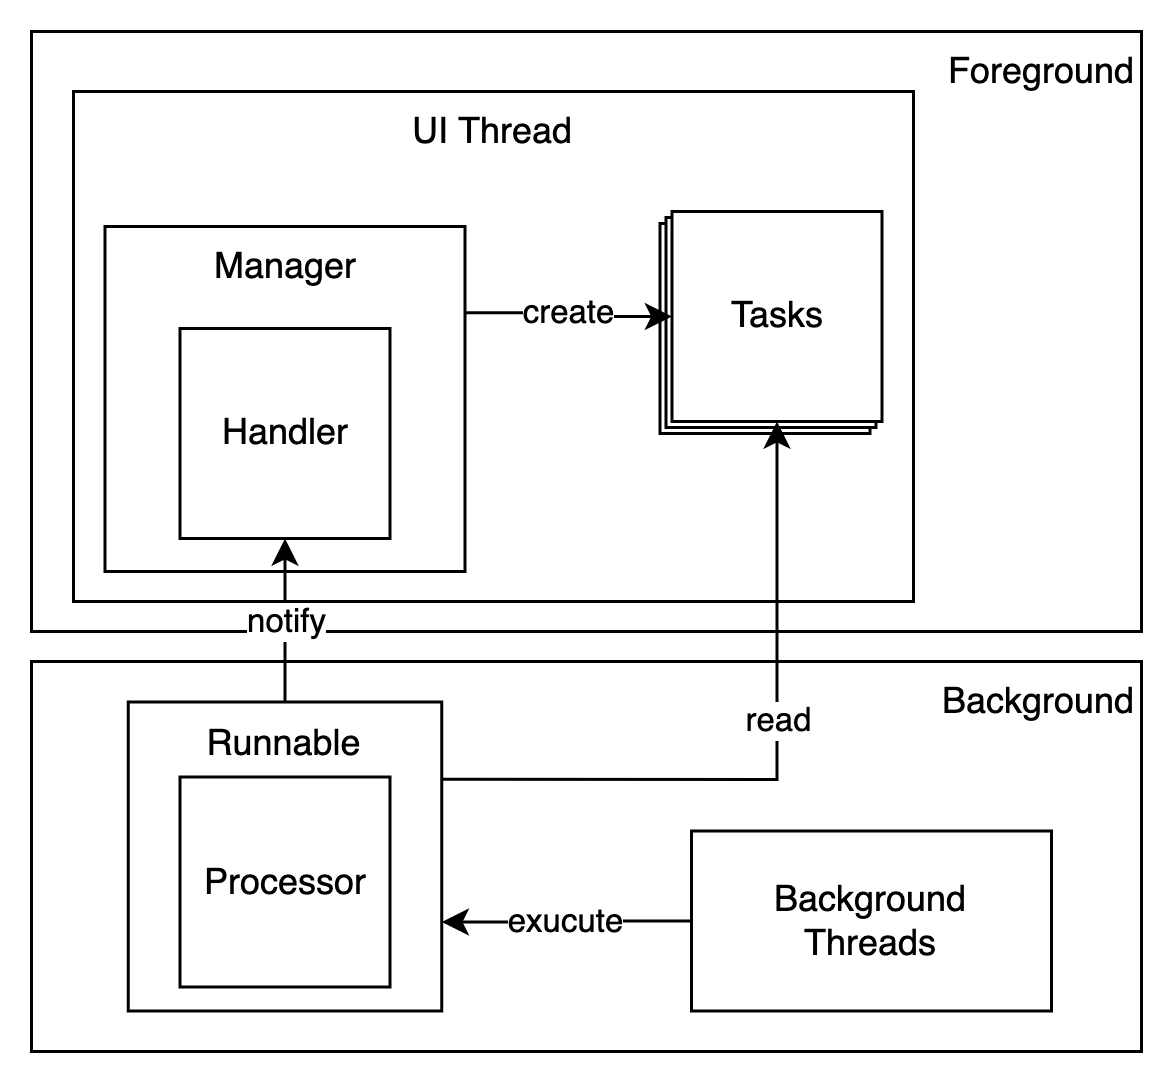
\includegraphics[width=3in]{images/chapter2/thread-overview.png}
            \caption{Threading Overview}
            \label{thread-overview}
        \end{figure}

        A working thread is separated from the UI thread to avoid freezing application,
            and it is called worker thread or background thread.
            This thread is able to process a long-running task in the background without interrupting the UI thread.
        In addition, the priority of the thread can be set from -20 to 19---the lowest priority is 19 and the highest priority is -20.
            The default value of background threads priority is 10,
            and the default value of foreground threads is -2 \cite{ANDROID-02}.

        UI thread and background thread run on different threads,
        thus a Handler is needed when there is communication between these threads.
        For example, as shown in Figure \ref{thread-overview},
        processes are divided into two parts: foreground and background.
        Tasks are created by a manager which is running on the UI thread.
        Then, Runnable, a component that can be run by background threads, will read tasks.
        After that, Runnable will be executed by background threads.
        Finally, Runnable will notify the manager through Handler.

    \section{Distance Calculation}\label{sectionDistanceCalculation}
        According to Gurucharan \cite{SOCIAL-DISTANCING-DETECTION}, to measure a distance between 2 people, the reference points of them are used for calculation.
        The reference point is the coordination of the 2 people, which is the centre of the detection frame.
        The calculation formula is based on Euclidean distance:

        \begin{equation*}
            d = \sqrt{(a_{0}-b_{0})^{2}+(D/c)\times(a_{1}-b_{1})^{2}}
        \end{equation*}

        \begin{equation*}
            c = \frac{a_{1}+b_{1}}{2}
        \end{equation*}

        However, a three-dimensional space is captured into a two-dimensional image,
        so depth and perspective can be seen in Figure \ref{distanceCalculation}.
        Thus, a couple of variables are added into the formula.
        The first variable is $D$, which is the diagonal of the image.
        The second variable is $c$, which is a calibration.
        These two variables will determine the depth of people in the image.

        \begin{figure}[h!]
            \centering
            \begin{subfigure}{.5\textwidth}
              \centering
              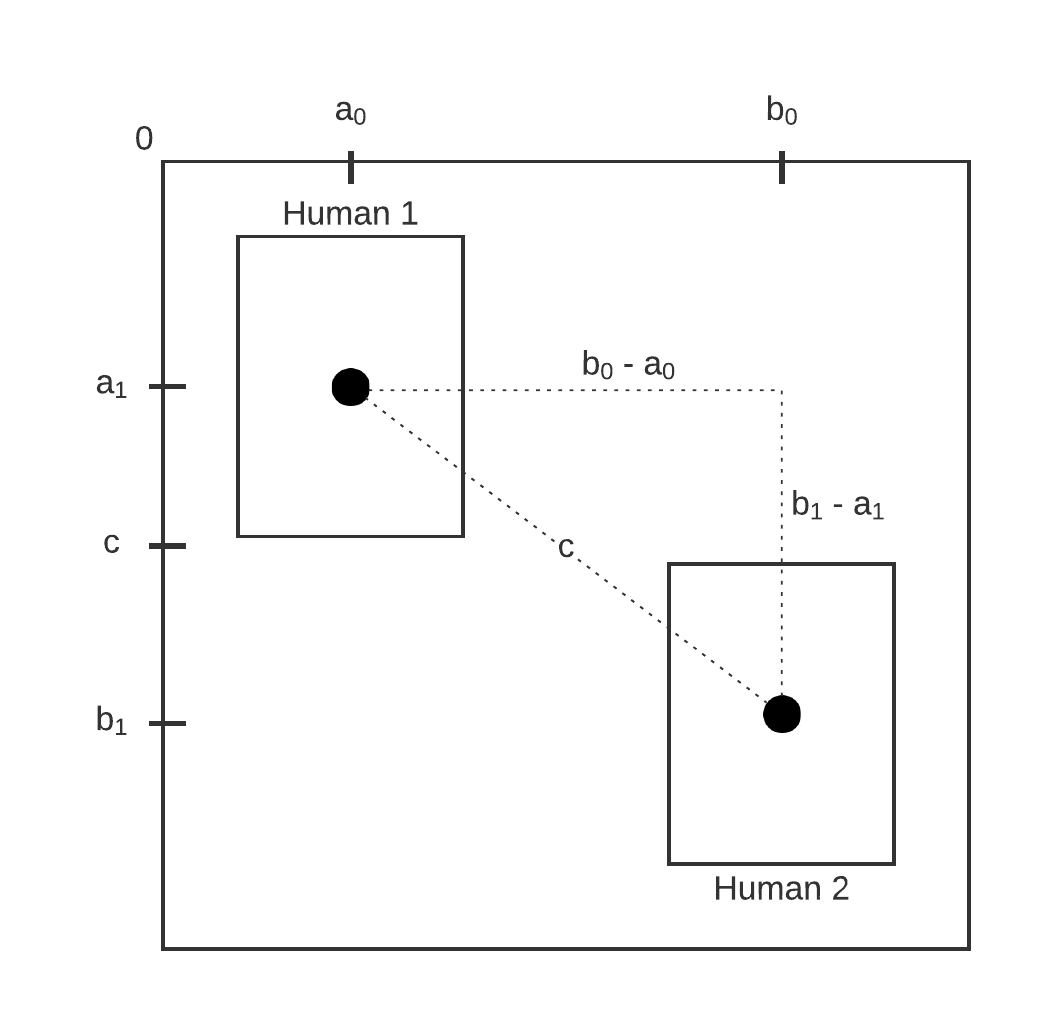
\includegraphics[width=2.5in]{images/chapter2/distance.png}
              \caption{Distance calculation}
              \label{distanceCalculation}
            \end{subfigure}%
            \begin{subfigure}{.5\textwidth}
              \centering
              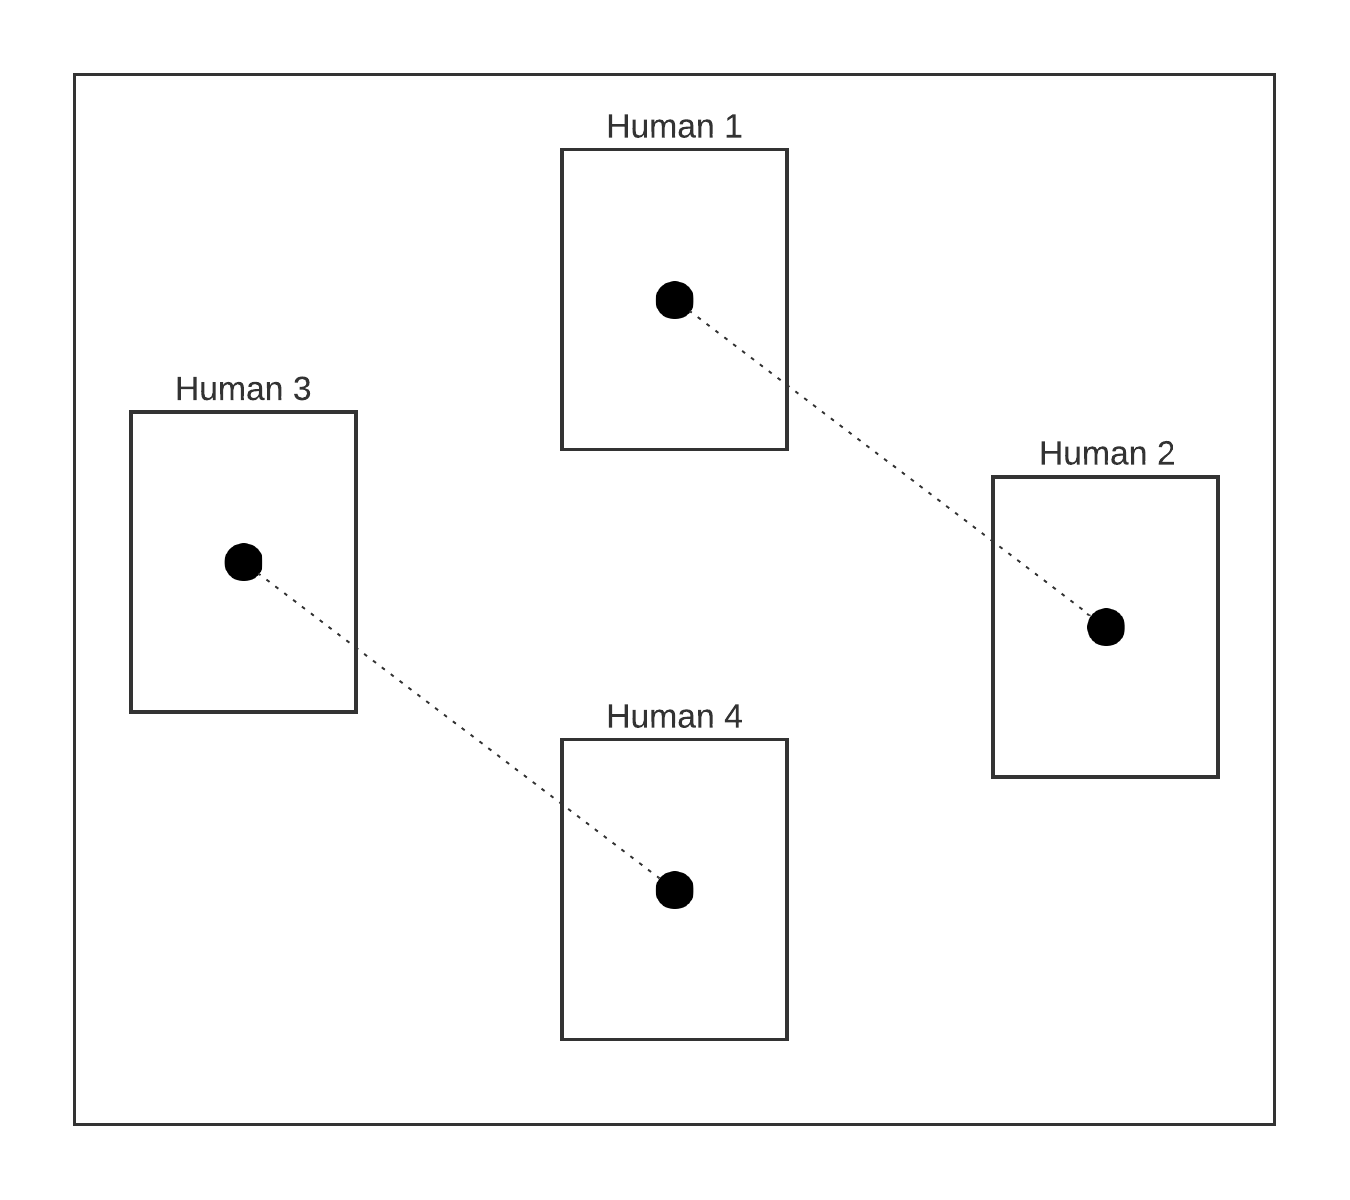
\includegraphics[width=2.5in]{images/chapter2/two-distances.png}
              \caption{A difference of 2 distances}
              \label{twoDistances}
            \end{subfigure}
            \caption{Determining Social Distancing}
            \label{determiningConcept}
        \end{figure}

        For example, according to Figure \ref{twoDistances},
        if the distance is calculated without calibration, the distance between 2 groups of people will be the same.
        Naturally, the distance between Human1 and Human2 must be further than the distance between Human3 and Human4.

    \section{Related Work}
        \subsection{Object Detector}
            Object Detector is an Android application\footnote{https://play.google.com/store/apps/details?id=com.tecomen.android.objectdetector},
            which is able to detect objects through a camera.
            This application is implemented by a deep learning library from TensorFlow \cite{tensorflow2015-whitepaper} with
            MobileNet model\footnote{https://tfhub.dev/tensorflow/lite-model/ssd\_mobilenet\_v1/1/metadata/1?lite-format=tflite} \cite{mobilenet} \cite{ssd} and COCO dataset \cite{coco-dataset}. There are two modes in this application,
            which are detection mode and classification mode.
            The processing time of each frame is 250 to 300 milliseconds.
            The screenshot of the application can be seen in Figure \ref{appendix:obj-detector}.

        \subsection{TensorFlow Object Detection}
            TensorFlow Object Detection is an object detection application\footnote{https://play.google.com/store/apps/details?id=org.tensorflow.detect},
            which is run on the Android operating system.
            TensorFlow's library is used in this application, along with the MobileNet model.
            This application is able to detect objects in real-time from the camera.
            The screenshot of the application can be seen in Figure \ref{appendix:ts-obj-detection}.


        \subsection{Computer Vision Detection}
            Computer Vision Detection application operates on the Android operating system\footnote{https://play.google.com/store/apps/details?id=com.pobeda.ivan.opencvdetect}.
            This application is able to process real-time video from a live camera,
            and OpenCV is used as a library \cite{opencv_library}.
            There are 12 options of algorithms, such as colour detector, canny detector, motion detector, and shape detector.
            Besides, this application is able to detect human faces and smiling faces.
            This application is able to process around 13 frames per second.
            The screenshot of the application can be seen in Figure \ref{appendix:cv-detection}.

        \subsection{Real Time Object Detection and Tracking Using Deep Learning and OpenCV}
            Demonstrates and explains how objects are detected and tracked in real-time \cite{related-work-1}.
            Objects are detected by using Single Shot Detector algorithm (SSD),
            which is trained with MobileNet.
            In this paper, many techniques are used to enhance the performance of the detection.
            At the first step, frames are extracted from the camera.
            Then, a local mean algorithm is applied to filter noise,
            and reduce the complexity and computing time of preprocessing.
            In addition, background subtraction is used to localise the detected object in the frame.
            The detected object is considered as a foreground object,
            and it is separated from background for further processing.
            Furthermore, the object will be tracked after the object is detected,
            which reduce the processing time because detection can be processing a few frames,
            while tracking the object can be processed faster.
            The result of this research shows that SSD can process the given image faster than YOLO model,
            and SSD can detect the object with confidence over 98\%.
            In addition, this work shows that humans can be detected with an accuracy of 99\%